\documentclass[tikz,border=2pt,11pt]{standalone}
\usetikzlibrary{arrows.meta}
\usetikzlibrary{patterns}
\usetikzlibrary{calc}
\usepackage{amsmath}
\usepackage{amssymb}
\usepackage{tikz}
\usepackage{xcolor}
\def\expandafter\UrlBreaks\expandafter{\UrlBreaks\do\-}
\newcommand{\T}{\mathbb T}
\newcommand{\R}{\mathbb R}
\newcommand{\Z}{\mathbb Z}
\newcommand{\N}{\mathbb N}
\newcommand{\C}{\mathbb C}
\newcommand{\e}{\mathrm e}
\newcommand{\norm}[1]{\lVert #1\rVert}
\DeclareMathOperator{\sgn}{sgn}
\DeclareMathOperator{\supp}{supp}
\begin{document}
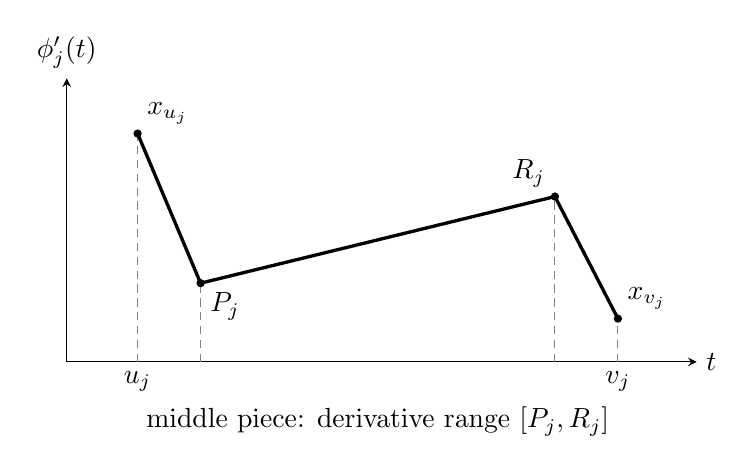
\begin{tikzpicture}[x=1cm,y=1cm,>=stealth]
 \draw[->] (0,0) -- (8,0) node[right] {$t$};
 \draw[->] (0,0) -- (0,3.6) node[above] {$\phi_j'(t)$};
 \draw[densely dashed,gray] (.9,0) -- (.9,2.9);
 \draw[densely dashed,gray] (1.7,0) -- (1.7,1.0);
 \draw[densely dashed,gray] (6.2,0) -- (6.2,2.1);
 \draw[densely dashed,gray] (7.0,0) -- (7.0,.55);
 \draw[very thick] (.9,2.9) -- (1.7,1.0) -- (6.2,2.1) -- (7.0,.55);
 \fill (.9,2.9) circle (1.5pt) node[above right] {$x_{u_j}$};
 \fill (1.7,1.0) circle (1.5pt) node[below right] {$P_j$};
 \fill (6.2,2.1) circle (1.5pt) node[above left] {$R_j$};
 \fill (7.0,.55) circle (1.5pt) node[above right] {$x_{v_j}$};
 \node[below] at (.9,0) {$u_j$};
 \node[below] at (7.0,0) {$v_j$};
 \node[below,align=center] at (3.95,-.45) {middle piece: derivative range $[P_j,R_j]$};
\end{tikzpicture}
\end{document}
